\subsection{Fixed-Parameter Leave One Patient Out Benchmarks}
Logistic regression achieved the highest pooled AUC (0.874), while random forest achieved the highest accuracy (0.799), sensitivity (0.839), and F1 (0.808) among predictive models (Table~\ref{tab:building-lopo-results}). Logistic regression detected 132 of 161 positive records and correctly classified 118 of 158 controls; random forest detected 135 positive records and correctly classified 120 controls. Stacking had the highest specificity (0.772).

\begin{table}[tbp]
\centering
\footnotesize
\caption{Fixed-parameter Leave One Patient Out evaluation on 319 held-out predictions per model at threshold 0.5.}
\label{tab:building-lopo-results}
\begin{tabular}{@{}lrrrrrr@{}}
\toprule
Model & Accuracy & ROC--AUC & Sensitivity & Specificity & F1 & FNR \\
\midrule
Logistic regression & 0.784 & \textbf{0.874} & 0.820 & 0.747 & 0.793 & 0.180 \\
Random forest & \textbf{0.799} & 0.857 & \textbf{0.839} & 0.759 & \textbf{0.808} & \textbf{0.161} \\
XGBoost & 0.762 & 0.835 & 0.807 & 0.715 & 0.774 & 0.193 \\
LightGBM & 0.787 & 0.851 & 0.832 & 0.741 & 0.798 & 0.168 \\
Stacking & 0.787 & 0.865 & 0.801 & \textbf{0.772} & 0.791 & 0.199 \\
\midrule
Training-prior dummy & 0.505 & 0.000 & 1.000 & 0.000 & 0.671 & 0.000 \\
\bottomrule
\end{tabular}
\end{table}
The training-prior dummy's pooled AUC of 0.000 is a leave-one-out artefact: excluding a positive record lowers its training prevalence, while excluding a negative record raises it. Its pooled probabilities therefore rank the classes inversely, even though every thresholded prediction is positive. The value is not evidence of useful discrimination.

The single LOPO run compares fixed pipelines using the same excluded records; it does not estimate between-seed variability or the performance of a nested model-selection procedure.

\subsection{Optuna-Tuned Leave One Patient Out Benchmarks}
All five predictive families completed 319 outer folds with 20 Optuna trials and three stratified inner folds per outer training set. The source-data signature, feature count, seed, threshold, and dependency versions were identical across tuned runs. Table~\ref{tab:tuned-lopo-results} reports pooled held-out performance; hyperparameters were selected separately within each outer fold.

\begin{table}[tbp]
\centering
\footnotesize
\setlength{\tabcolsep}{4pt}
\caption{Optuna-tuned Leave One Patient Out evaluation: 319 held-out predictions per family, RFE--CART with 20 source predictors, and threshold 0.5. Bold marks the best predictive-family value in each rate column. FN: number of missed gallstone cases out of 161.}
\label{tab:tuned-lopo-results}
\begin{tabular}{@{}lrrrrrrr@{}}
\toprule
Model & Accuracy & ROC--AUC & Sensitivity & Specificity & F1 & FNR & FN \\
\midrule
Logistic regression & \textbf{0.787} & \textbf{0.868} & \textbf{0.826} & 0.747 & \textbf{0.796} & \textbf{0.174} & 28 \\
Random forest & 0.774 & 0.842 & 0.807 & 0.741 & 0.783 & 0.193 & 31 \\
XGBoost & 0.784 & 0.851 & \textbf{0.826} & 0.741 & 0.794 & \textbf{0.174} & 28 \\
LightGBM & \textbf{0.787} & 0.840 & 0.814 & \textbf{0.759} & 0.794 & 0.186 & 30 \\
Stacking & 0.784 & 0.862 & 0.807 & \textbf{0.759} & 0.790 & 0.193 & 31 \\
\bottomrule
\end{tabular}
\end{table}

Tuned logistic regression retained the highest AUC (0.868) and F1 (0.796), with accuracy 0.787 and sensitivity 0.826. It detected 133 of 161 cases and correctly classified 118 of 158 controls. XGBoost matched its sensitivity and false-negative count (28), but had lower AUC (0.851) and one additional false positive (41 versus 40). LightGBM matched the highest accuracy (0.787), while LightGBM and stacking shared the highest specificity (0.759). Random forest achieved AUC 0.842 and sensitivity 0.807. Stacking did not exceed logistic regression in discrimination or sensitivity; only its logistic meta-learner was tuned, with fixed base-model settings.

\subsection{Changes Relative to Fixed Configurations}
XGBoost showed the largest positive change relative to its historical fixed benchmark: AUC increased from 0.835 to 0.851, accuracy from 0.762 to 0.784, and sensitivity from 0.807 to 0.826; false negatives decreased from 31 to 28. Logistic regression's AUC decreased from 0.874 to 0.868, although accuracy increased slightly and one fewer positive record was missed. Random forest's AUC decreased from 0.857 to 0.842, with five additional false negatives (26 to 31). LightGBM's accuracy was unchanged, but AUC decreased from 0.851 to 0.840 and false negatives increased from 27 to 30. Stacking's AUC decreased from 0.865 to 0.862; one fewer false negative was offset by two additional false positives.

These differences are descriptive rather than evidence that tuning alone caused the changes. The historical fixed run used scikit-learn 1.7.1, whereas the tuned runs used 1.9.1; NumPy and pandas versions also differed. Although the cohort and outer record exclusions were shared, a controlled estimate of tuning's effect requires refitting the fixed configurations in the tuned environment. No significance test or confidence interval was calculated. Optimising inner-fold AUC did not consistently improve outer discrimination or classification at threshold 0.5, and the search budget does not establish globally optimal parameters.

\subsection{Recurring Classification Errors in Fixed Models}
Source record 117 was a false negative in four of the five predictive LOPO models. Records 291 and 316 were false positives in all five. These retrospectively identified examples indicate disagreement between observed labels and predictions across model families, without establishing clinical causes or labelling errors. They support inspecting common failure cases in addition to aggregate discrimination and classification metrics.

\subsection{SHAP and LIME Visualisation}
Figure~\ref{fig:xai-global} summarises the 20 sampled held-out explanations from the tuned logistic models. The largest mean absolute SHAP contributions were associated with the source fields \texttt{bm} (0.208), CRP (0.173), extracellular-fluid/total-body-water ratio (0.071), vitamin D (0.068), weight (0.065), and extracellular water (0.056). The ordering describes this small sample and the fold-specific models, rather than a population-level ranking. Higher recorded CRP values generally contributed towards the absent class within these fitted models; this association does not imply a protective biological effect.

\begin{figure}[tbp]
\centering
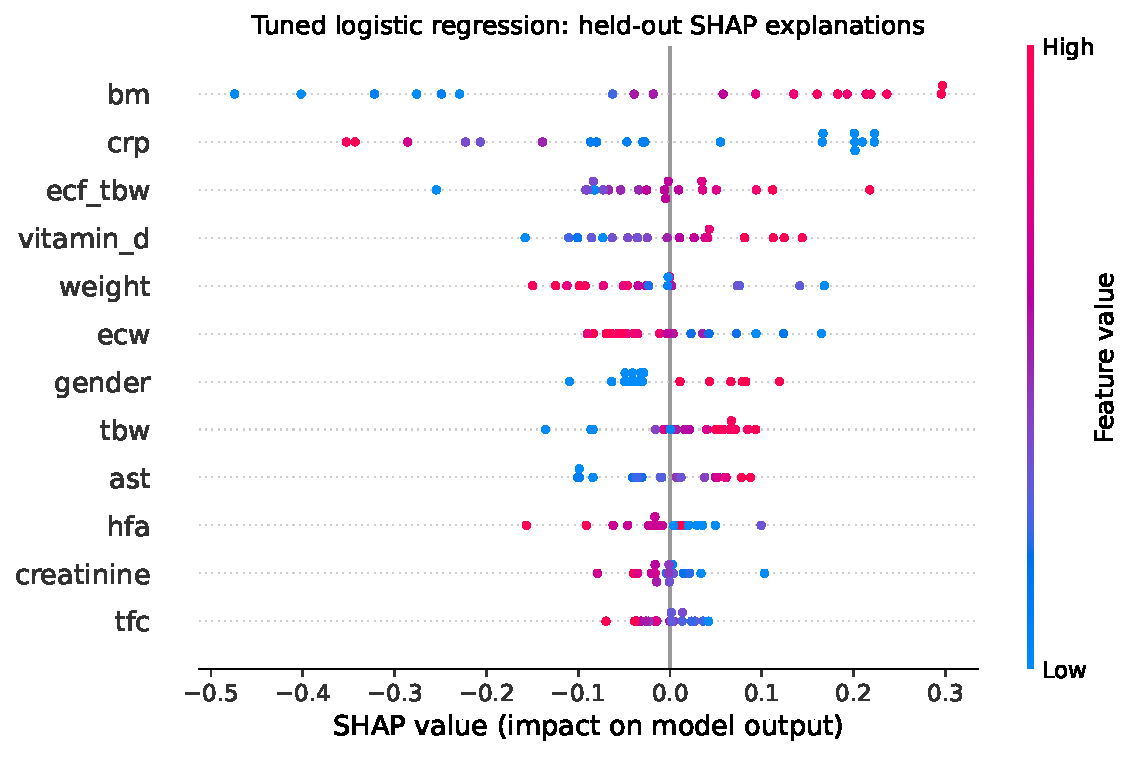
\includegraphics[width=0.88\linewidth]{figures/xai/global_shap.pdf}
\caption{Kernel SHAP summary for 20 sampled excluded records from tuned logistic Leave One Patient Out models. Each point uses its own outer-fold model and training-only background. Positive values increase the predicted probability of gallstones; negative values decrease it. Colour indicates the recorded feature value, and source-field labels follow the dataset schema. Features are ordered by sampled mean absolute contribution.}
\label{fig:xai-global}
\end{figure}

Figure~\ref{fig:xai-errors} compares SHAP and LIME for two confident errors. Source record 156 was a false negative with predicted probability 0.038; its largest displayed negative SHAP contributions included fluid ratio, \texttt{bm}, and vitamin D. Source record 178 was a false positive with predicted probability 0.995. These examples illustrate how multiple contributions can support an incorrect prediction despite aggregate discrimination. SHAP baselines were 0.443 and 0.413, respectively, and reconstruction from all feature contributions matched the saved probabilities. Only the eight largest contributions are displayed locally.

LIME surrogate $R^2$ was 0.423 for the false negative and 0.230 for the false positive, indicating limited local fidelity. For record 156, the surrogate prediction (0.160) also differed from the classifier probability (0.038). LIME condition weights and SHAP probability contributions have different meanings and should not be compared numerically. Agreement in direction is descriptive; correlated measurements and synthetic perturbations can produce unstable or implausible neighbourhoods.

\begin{figure}[p]
\centering
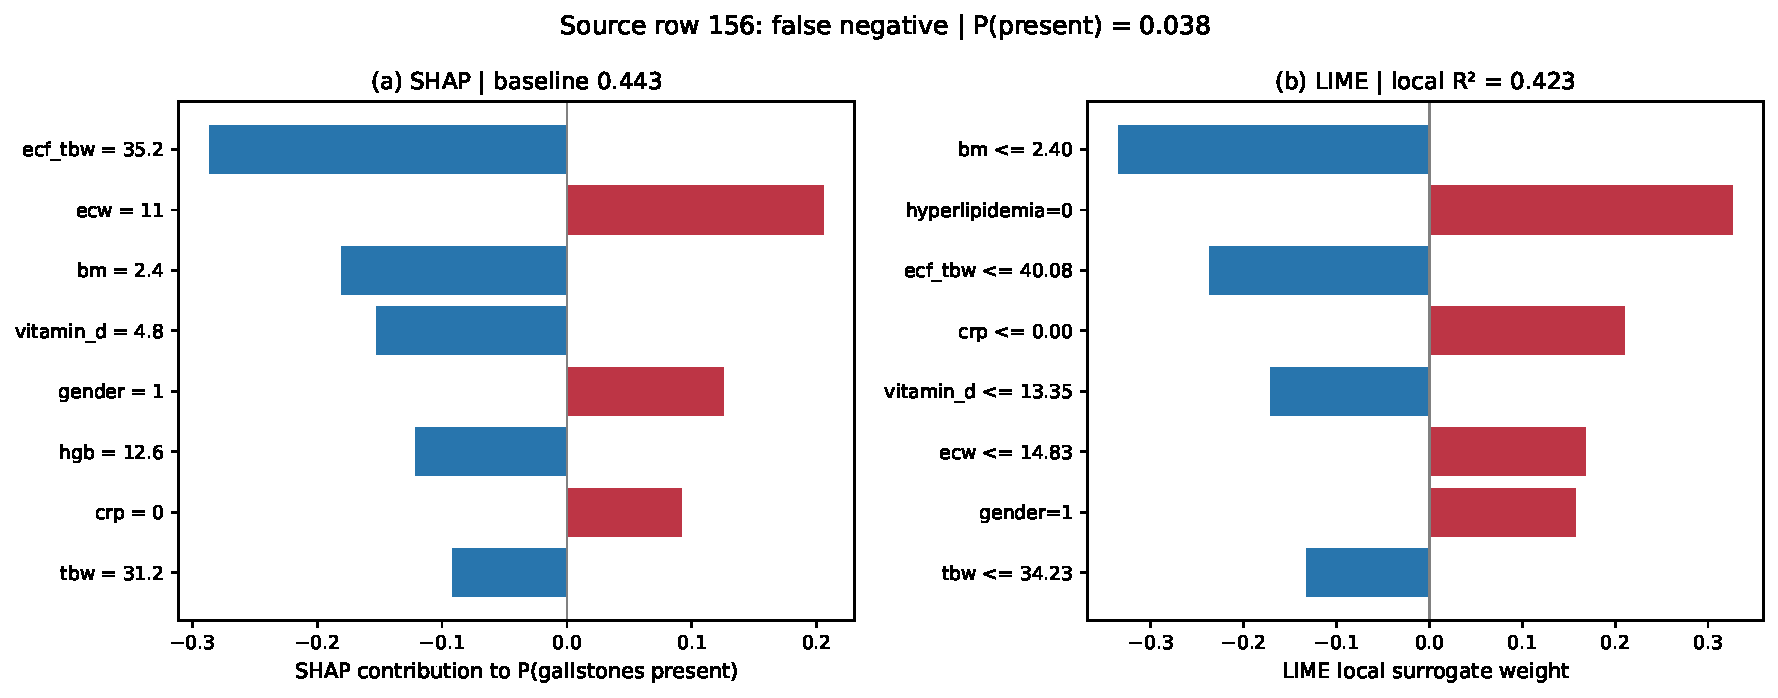
\includegraphics[width=\linewidth]{figures/xai/local_fn.pdf}
\par\medskip
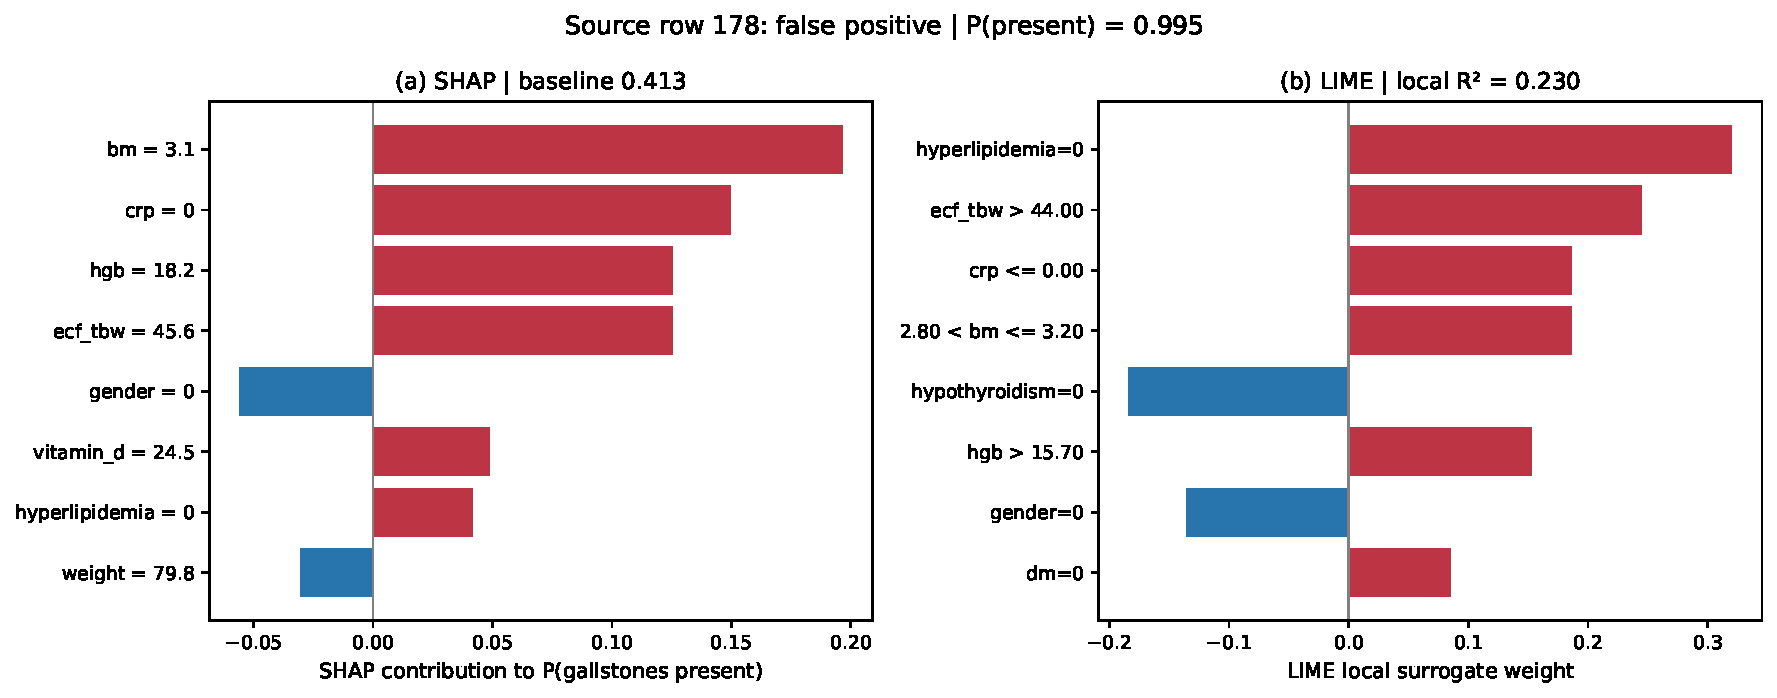
\includegraphics[width=\linewidth]{figures/xai/local_fp.pdf}
\caption{Local explanations of a retrospectively selected false negative (source row 156, top) and false positive (source row 178, bottom) from tuned logistic Leave One Patient Out evaluation. Left: the eight largest absolute SHAP contributions, labelled with recorded input values. Right: LIME condition weights and local surrogate fidelity. Red pushes towards gallstones present; blue pushes towards absent. Each excluded record was omitted from fitting, tuning, and explainer background construction. These selected examples do not estimate error prevalence.}
\label{fig:xai-errors}
\end{figure}

